%%%%%%%%%%%%%%%%%%%%%%%%%%%%%%%%%%%%%%%%%
% University/School Laboratory Report
% LaTeX Template
% Version 3.1 (25/3/14)
%
% This template has been downloaded from:
% http://www.LaTeXTemplates.com
%
% Original author:
% Linux and Unix Users Group at Virginia Tech Wiki 
% (https://vtluug.org/wiki/Example_LaTeX_chem_lab_report)
%
% License:
% CC BY-NC-SA 3.0 (http://creativecommons.org/licenses/by-nc-sa/3.0/)
%
%%%%%%%%%%%%%%%%%%%%%%%%%%%%%%%%%%%%%%%%%

%----------------------------------------------------------------------------------------
%	PACKAGES AND DOCUMENT CONFIGURATIONS
%----------------------------------------------------------------------------------------

\documentclass{article}

\usepackage[version=3]{mhchem} % Package for chemical equation typesetting
\usepackage{siunitx} % Provides the \SI{}{} and \si{} command for typesetting SI units
\usepackage{graphicx} % Required for the inclusion of images
\usepackage{natbib} % Required to change bibliography style to APA
\usepackage{amsmath} % Required for some math elements 

\setlength\parindent{15pt} % Removes all indentation from paragraphs

\renewcommand{\labelenumi}{\alph{enumi}.} % Make numbering in the enumerate environment by letter rather than number (e.g. section 6)

%\usepackage{times} % Uncomment to use the Times New Roman font

%----------------------------------------------------------------------------------------
%	DOCUMENT INFORMATION
%----------------------------------------------------------------------------------------

\title{Titanic: Machine Learning from Disaster \\ EECS 510} % Title

\author{Xiaoyang \textsc{Tan} \\ Zhaoyang \textsc{Liu} } % Author name


\date{\today} % Date for the report

\begin{document}
\maketitle
% If you wish to include an abstract, uncomment the lines below
% \begin{abstract}
% Abstract text
% \end{abstract}

%----------------------------------------------------------------------------------------
%	SECTION 1
%----------------------------------------------------------------------------------------

\section{Current work}

\subsection{Defining the problem}

\label{definitions}
	Information is given on a training set of passengers of the Titanic, for which the survival outcome is known. Given the training set information, the goal remains to predict each passenger?s survival outcome from a test set of passengers. The details of the challenge are given on the Kaggle site.
\newline
\newline
We will apply machine learning tools to solve the problem. In this case, we may consider approaches based on random forests. And will use Python package to plot the result. The python package used includes:

\begin{itemize}
	\item NumPy
	\item Pandas
	\item SciKit-Learn
	\item SciPy
	\item StatsModels
	\item Patsy
	\item Matplotlib
\end{itemize}
 


\subsection{Analyze the data}
In the training dataset, there are 891 passengers. Each passenger has 12 attributes. Except the "passangerId" and "Survived" attribute, we need to consider 10 other attributes 
and predict the survival possibility.

\subsubsection{Take care of missing values}
The features \textit{Ticket} and \textit{Cabin} have many missing values and so can?t add much value to our analysis. To handle this we will drop them from the data frame to preserve the integrity of our dataset. What's more, we will remove NaN values from every remaining column. Using \textbf{drop()} and \textbf{dropna()} function in could easily achieve goal. Now we have a clean and tidy dataset that is ready for analysis, we cut the dataset from 891 to 712, and get 8 effective attributes to do prediction.

\subsubsection{Graphical view of data}
The point of this competition is to predict if an individual will survive based on the features in the data like:
\begin{itemize}
	\item Traveling Class (called pclass in the data)
	\item Sex
	\item Age
\end{itemize}




\begin{figure}[h]
\begin{flushleft}
\hspace*{-1.2in}
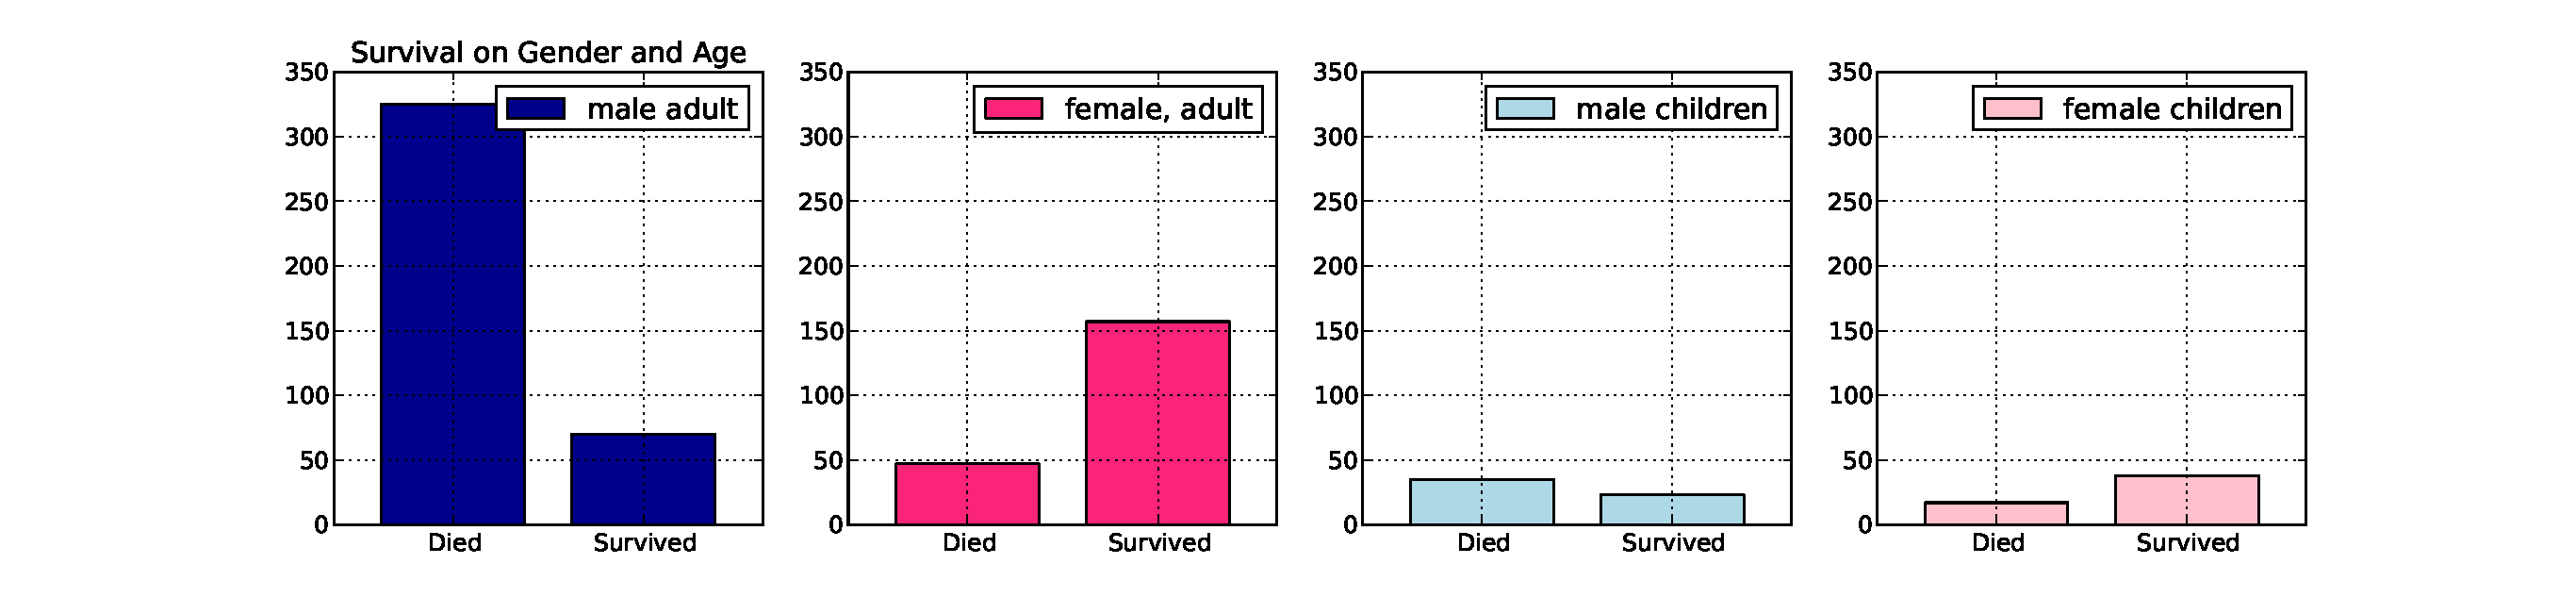
\includegraphics[scale=0.4]{eps/survival_gender_age.eps} % Include the image placeholder.png
\hspace*{-1.2in}
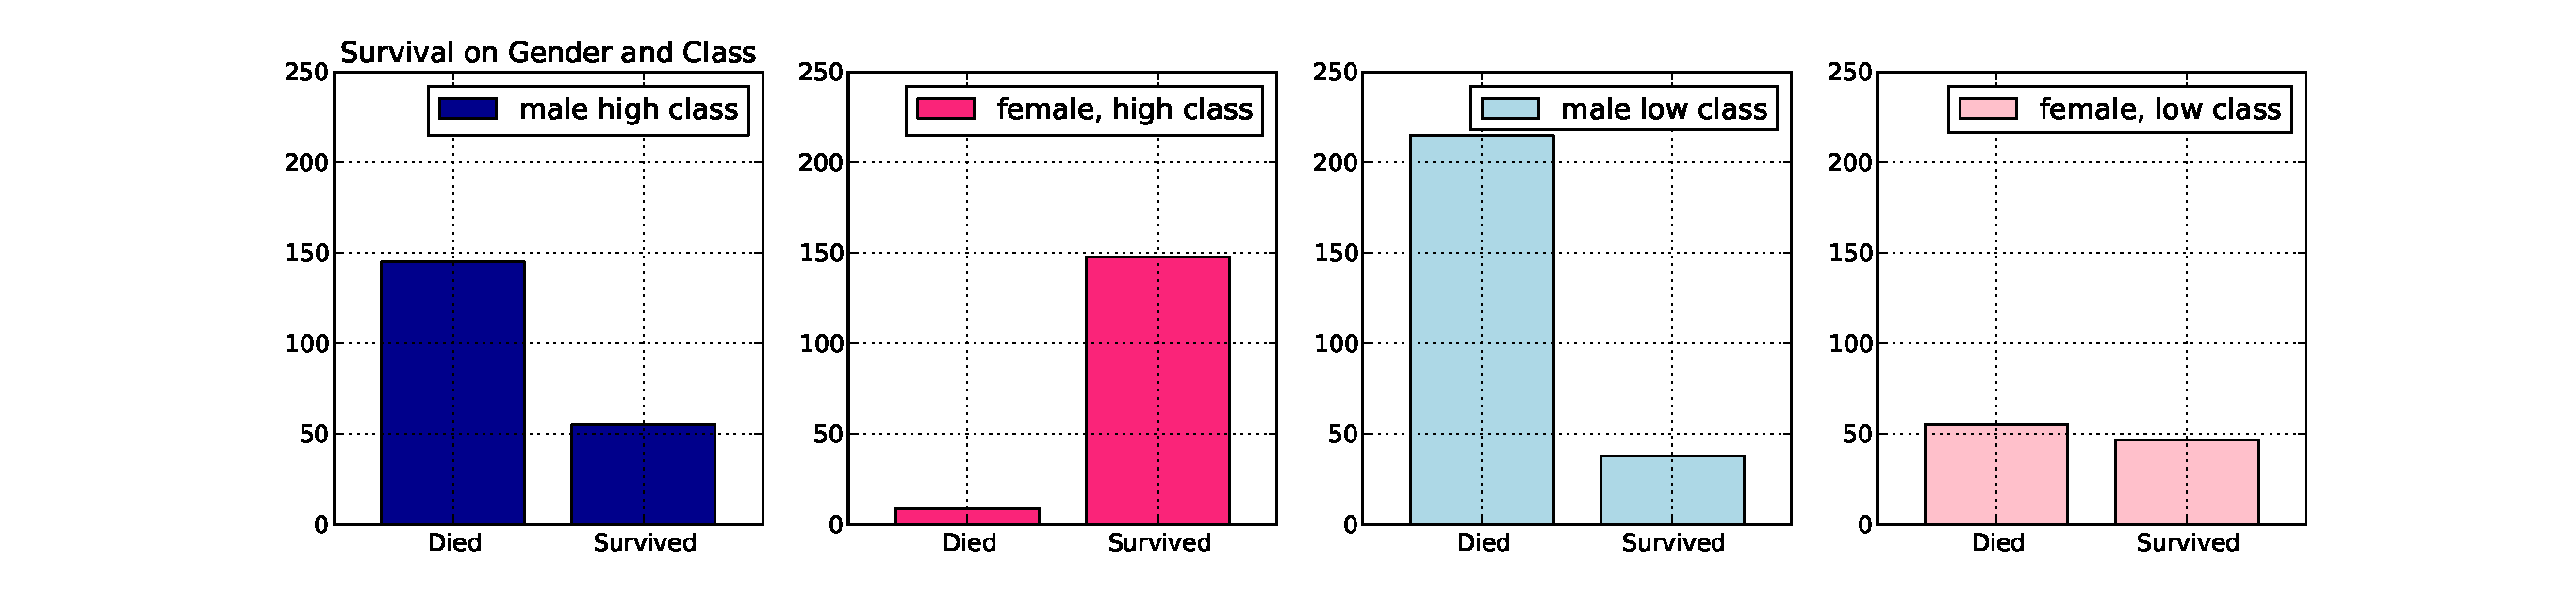
\includegraphics[scale=0.4]{eps/survival_gender_class.eps} 
\caption{Survival on gender, age and class}
\label {fig:test}
\end{flushleft}
\end{figure}

Figure~\ref{fig:test} shows the distribution of survival on gender age and class. ******


\subsection{Simple trying}
In the film, they tried to rescue women and children first, so a good guess would be on gender. From the graphical view of the data, it’s clear that although more men died and survived in raw value counts, females had a greater survival rate proportionally(~25\%), than men (~20\%).\\

After applying that all the female would survive, the survival rate become 36.36\%, which comes close to the original rate 38.38\%. However, we can refine our results by considering other variables.\\

We ruled out the age factor, as the survival rate doesn't change much with or without the involvement of age. Thus we split the fare class into four payments range and assumes that any group with more than half survivors will always be modeled to survive, while the rest will be mapped to death. The result is different from the previous one in that women in 3rd class who paid more than \$20 will not survive, which bring the survival rate closer to training set.

% \begin{figure}[h]
% \begin{flushleft}

% \hspace*{-1.2in}
% 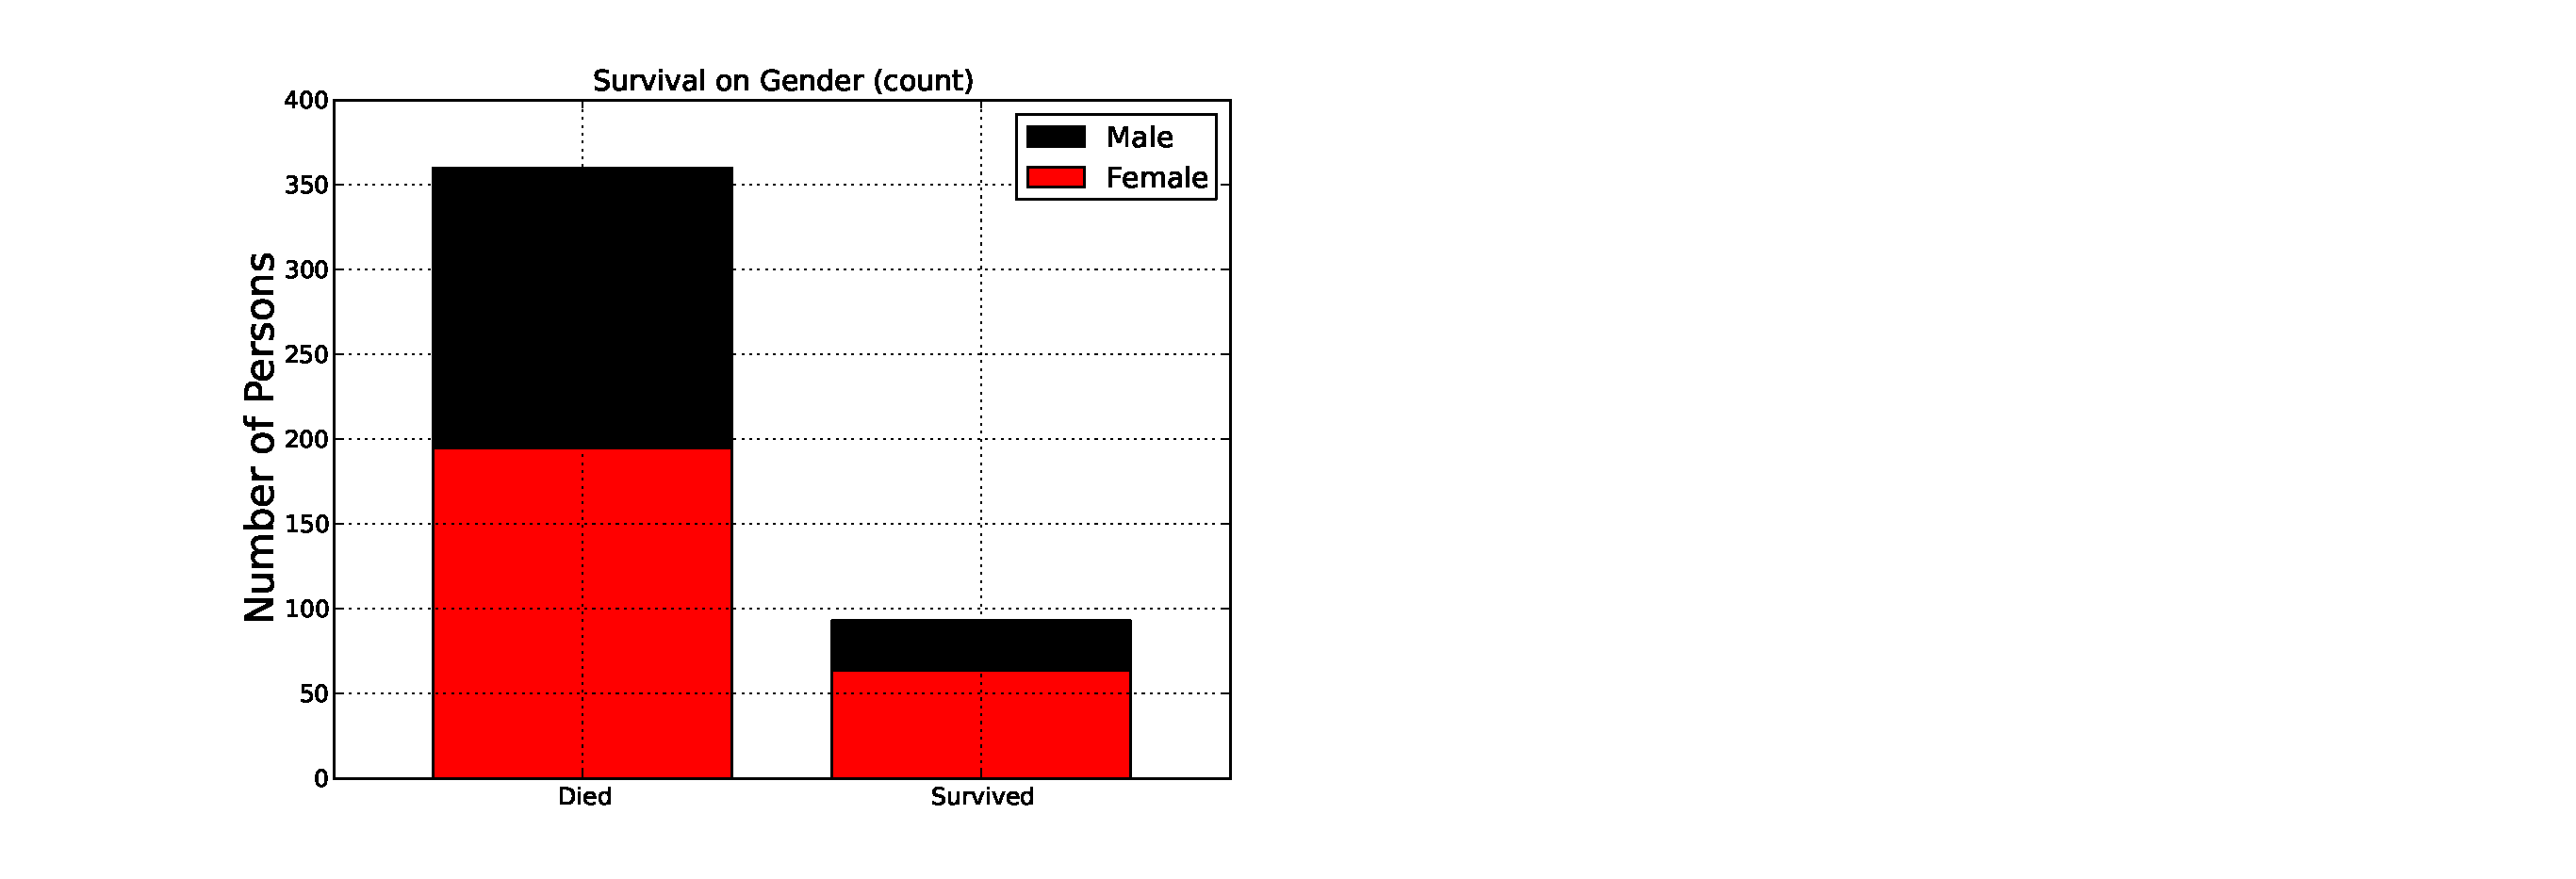
\includegraphics[scale=0.4]{eps/survival_gender_count.eps} 
% \caption{Survival on gender, age and class}
% \label {fig:test}
% \end{flushleft}
% \end{figure}

\subsection{Supervised machine learning}

In paticular, we are going to try \textbf{Logistic Regression}. In statistics, logistic regression or logit regression is a type of regression analysis used for predicting the outcome of a categorical dependent variable. We use python package \textbf{statsmodels} to build the model and use predictor variable including ``Plass'', ``Sex'', ``Embarked'', ``Age'', ``SibSp''. \\

First, we define our formula for our Logit regression. In the next cell we create a regression friendly dataframe that sets up boolean values for the categorical variables in our formula and lets our regression model know the types of inputs we're giving it. The model is then instantiated and fitted before a summary of the model's performance is printed. In the last cell we graphically compare the predictions of our model to the actual values we are trying to predict, as well as the residual errors from our model to check for any structure we may have missed. The result as Table~\ref{tab:logit} shows.


\begin{table}[h]
  \caption{Logit Regression Results}
\begin{tabular}{| l | l | l | l | l | l | l |}
  \hline
   & coef & std err & z & P \textgreater z & [95.0\% Conf. & Int.] \\
   \hline
C(Pclass)[T.2]    &  -1.2673    &  0.299   &  -4.245    &  0.000     &   -1.852  &  -0.682 \\
  \hline
C(Pclass)[T.3]    &  -2.4966    &  0.296   &  -8.422    &  0.000     &   -3.078  &  -1.916 \\
  \hline
C(Sex)[T.male]    &  -2.6239    &  0.218   & -12.060    &  0.000     &   -3.050  &  -2.197 \\
  \hline
C(Embarked)[T.Q]  &  -0.8351    &  0.597   &  -1.398    &  0.162     &   -2.006  &   0.335 \\
  \hline
C(Embarked)[T.S]  &  -0.4254    &  0.271   &  -1.572    &  0.116     &   -0.956  &   0.105 \\
  \hline
Age               &  -0.0436    &  0.008   &  -5.264    &  0.000     &   -0.060  &  -0.027 \\
  \hline
SibSp             &  -0.3697    &  0.123   &  -3.004    &  0.003     &   -0.611  &  -0.129 \\
  \hline

\end{tabular}
\label {tab:logit}
\end{table}





\begin{figure}[h]
\begin{flushleft}
\hspace*{-1.2in}
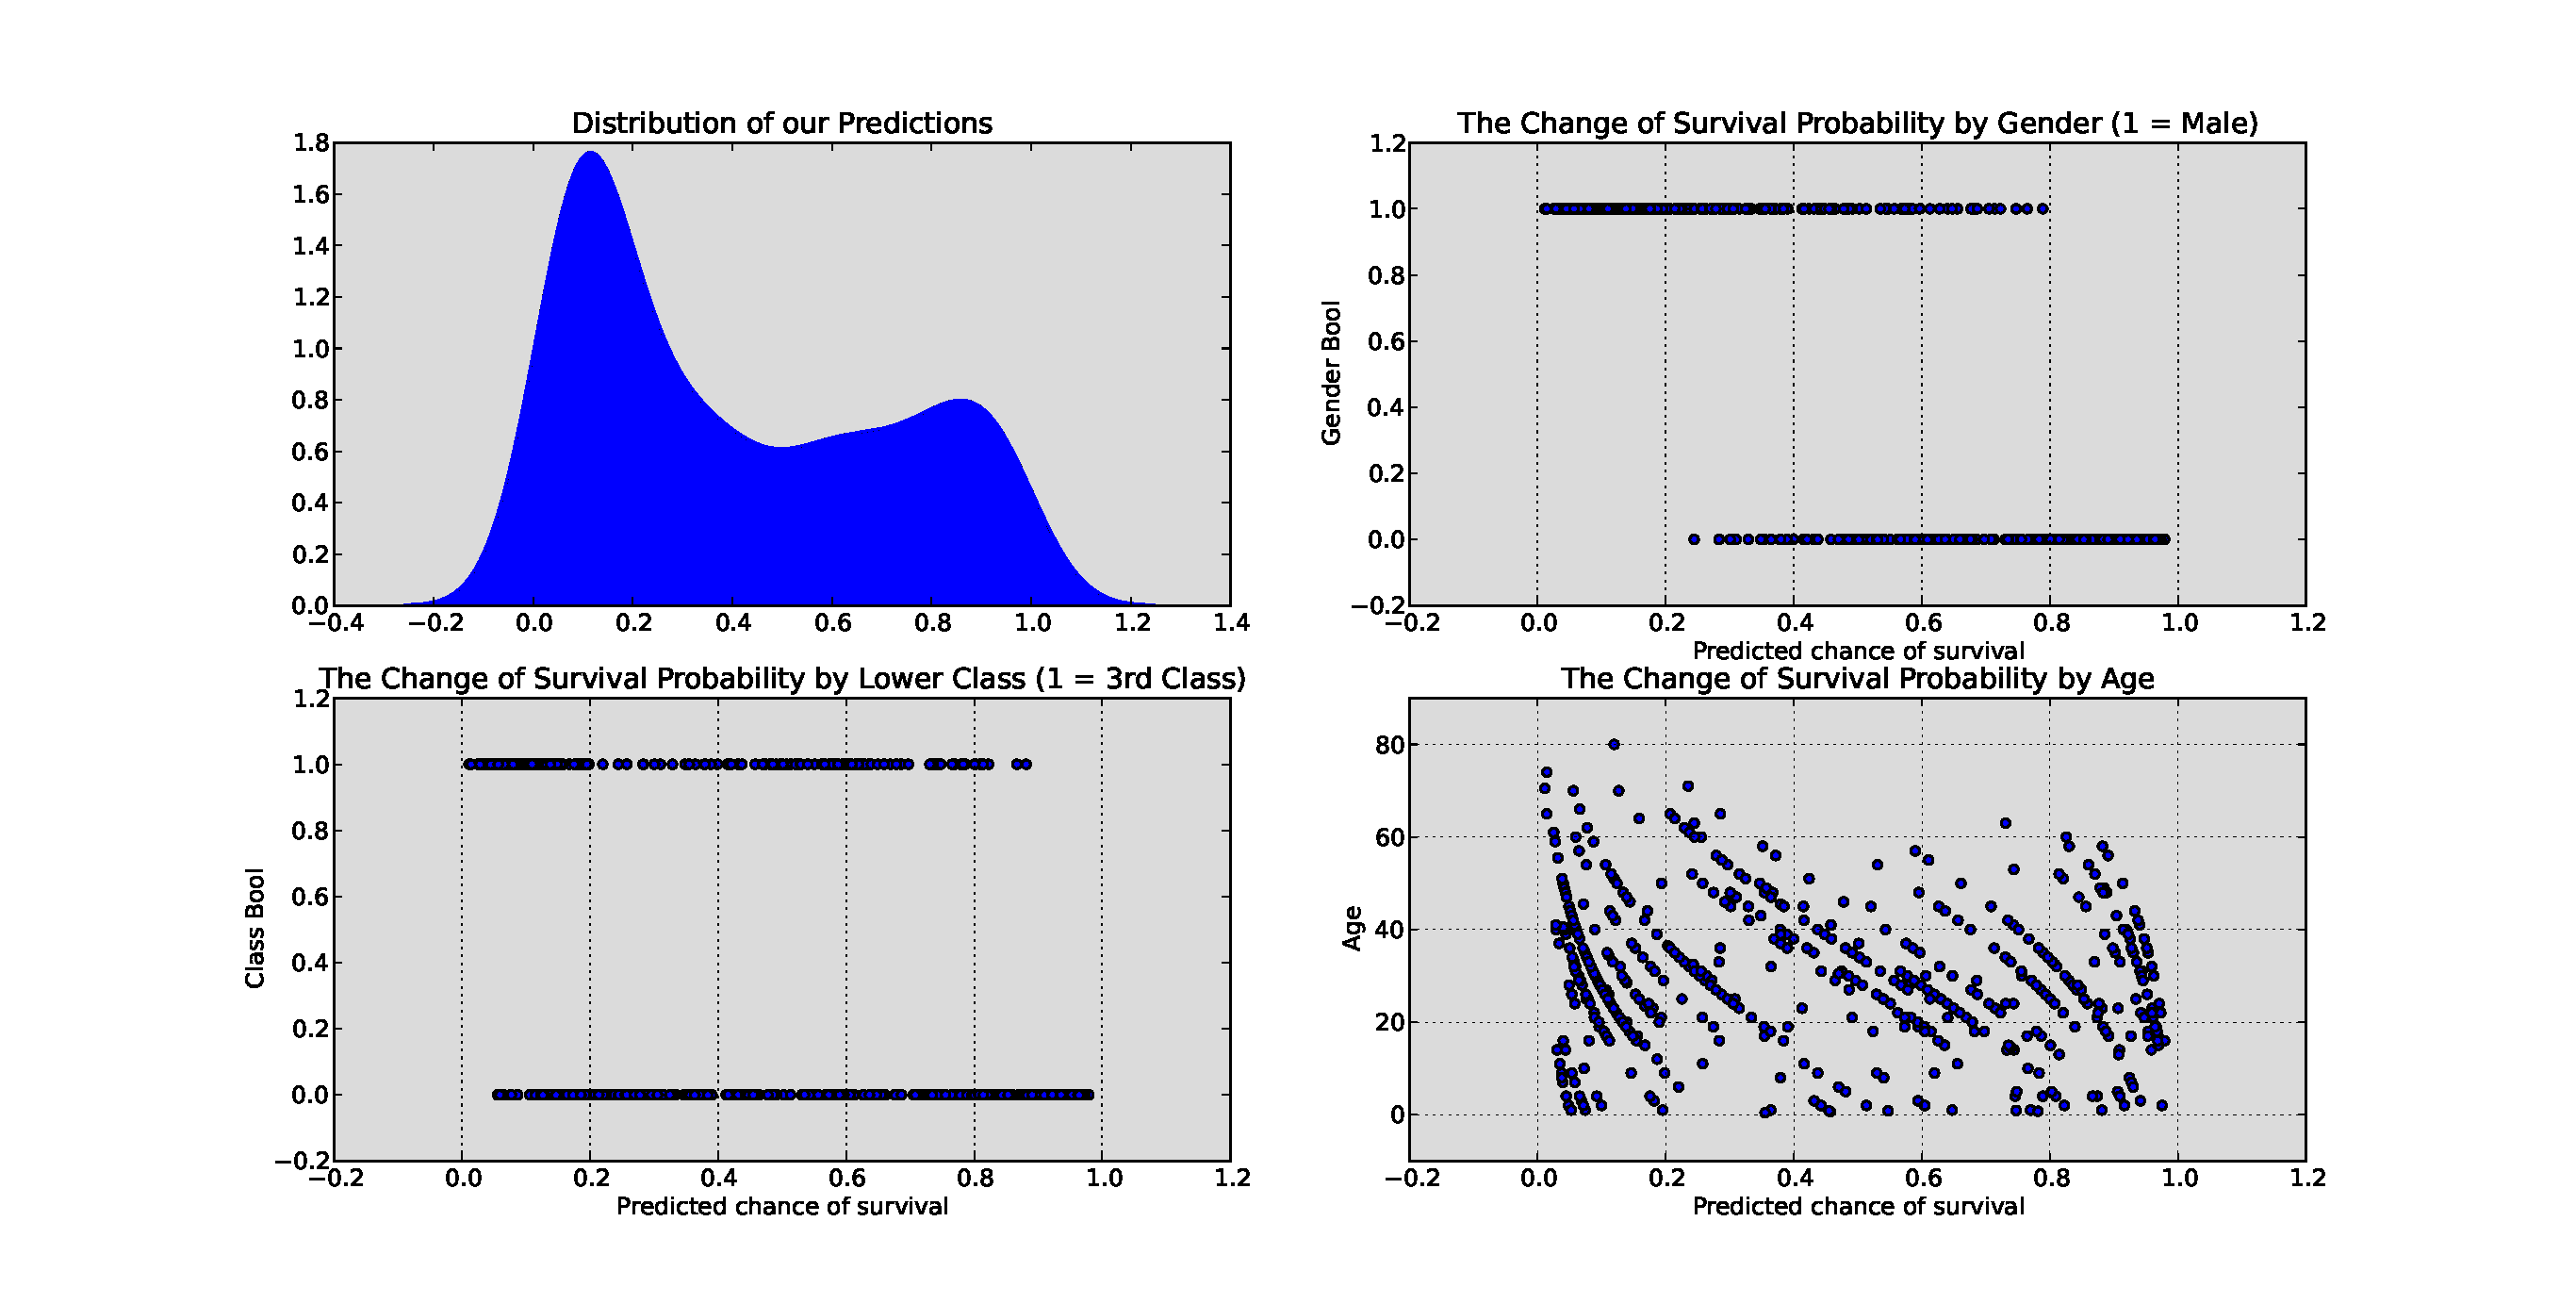
\includegraphics[scale=0.4]{eps/prediction.eps} % Include the image placeholder.png
\caption{Prediction from Logit Regression}
\label {fig:pre}
\end{flushleft}
\end{figure}


The Figure~\ref{fig:pre} shows the distribution of our predictions. The second graph also indicates that male has a higher possibility of died while female prefer to survive. This is consistent to our previous observations. Also, We can see from the third graph that ship class has slight effect on the prediction result. \\

After applying the model on the test data, we get an output file. Submitting this file shows that we got 77.03\%.


% (a dependent variable that can take on a limited number of values, whose magnitudes are not meaningful but whose ordering of magnitudes may or may not be meaningful) based on one or more predictor variables. That is, it is used in estimating empirical values of the parameters in a qualitative response model. The probabilities describing the possible outcomes of a single trial are modeled, as a function of the explanatory (predictor) variables, using a logistic function

%----------------------------------------------------------------------------------------
%	SECTION 2
%----------------------------------------------------------------------------------------

\section{Next step}
Next step is to try use support vector machine and random forest methods to make prediction.


\subsection{SVM}

The logit model we just implemented performed well and showed exactly where to draw our decision boundary or our 'survival cut off'. But when a straight line doesn't cut it, we have to apply a more complex decision boundary like a wave, circle, or maybe some sort of strange polygon, which would describe the variance observed in our sample better than a line. If the prediction of survival were based on age, that could be a linear decision boundary, meaning each additional time you've gone around the sun you were 1 unit more or less likely to survive. But it could be easy to use a curve, where a young healthy people would stand a better  chance of survival than elderly or youth. \\

To get around the fact that our logit model can only evaluate a linear decision boundary, we could transform our logit equation from expressing a linear relationship like so:\\

{\centering
$Survived=\beta_0+\beta_1Pclass+\beta_2Sex+\beta_3Age+\beta_4SibSp+\beta_5Parch+\beta_6Embarked$}\\

We'll represent this for convenience as: $y=x$ and transform that into a non-linear relationship: $log(y)=log(x)$. An easy way to visualize this by looking at a graph an exponential relationship. Here if we transformed the non-linear by taking the log of our equation, $log(y)=log(x^3)$ we would get a graph like this: 
\\
\begin{figure}[ht]
\begin{minipage}[b]{0.45\linewidth}
\centering
\includegraphics[width=2.5in]{eps/X^3.eps}
\caption{$x^3$}
\label{fig:figure1}
\end{minipage}
\hspace{0.2cm}
\begin{minipage}[b]{0.45\linewidth}
\centering
\includegraphics[width=2.5in]{eps/log_X^3.eps}
\caption{$log(x^3)$}
\label{fig:figure2}
\end{minipage}
\end{figure}
\\

This process of Support Vector Machine transforms models and expresses them in a different mathematical plane. We then implemented SVM model and examined the results after the SVM transforms the equation into three different mathematical planes. The first is linear, and is similar to our logic model. Next is a blank transformation and finally an exponential, polynomial transformation.\\

\begin{figure}[ht]
\begin{minipage}[b]{0.45\linewidth}
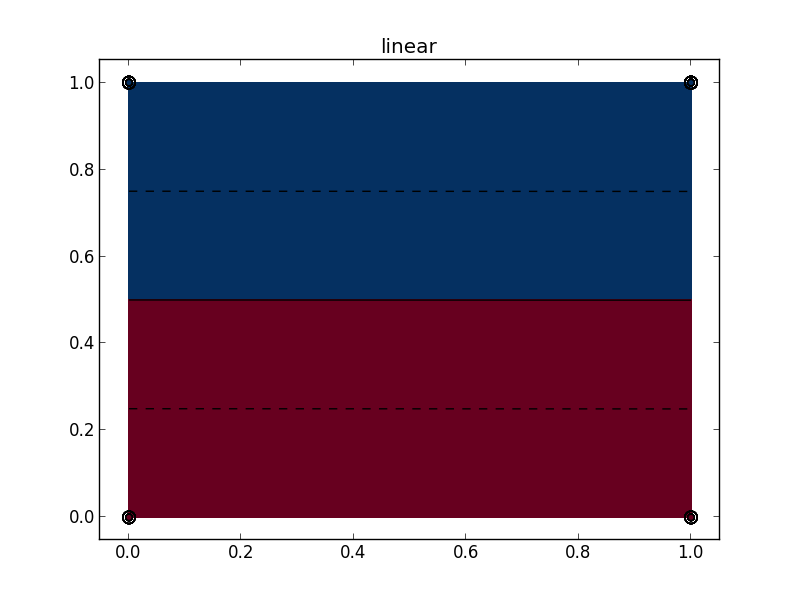
\includegraphics[width=2.4in]{eps/test_SVM_linear.png}
\caption{linear kernel}
\label{fig:figure1}
\end{minipage}
\begin{minipage}[b]{0.45\linewidth}
\centering
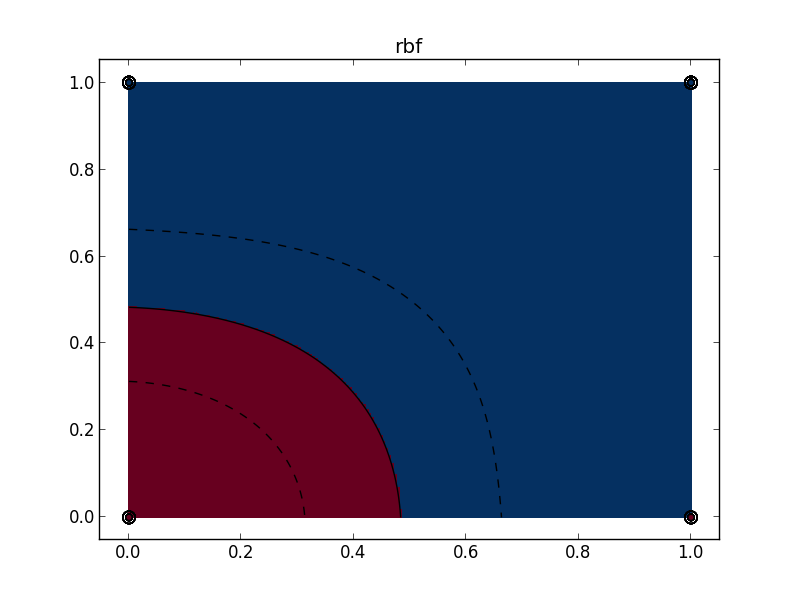
\includegraphics[width=2.4in]{eps/test_SVM_rbf.png}
\caption{rbf kernel}
\label{fig:figure2}
\end{minipage}
\end{figure}

\begin{figure}[h]
\centering
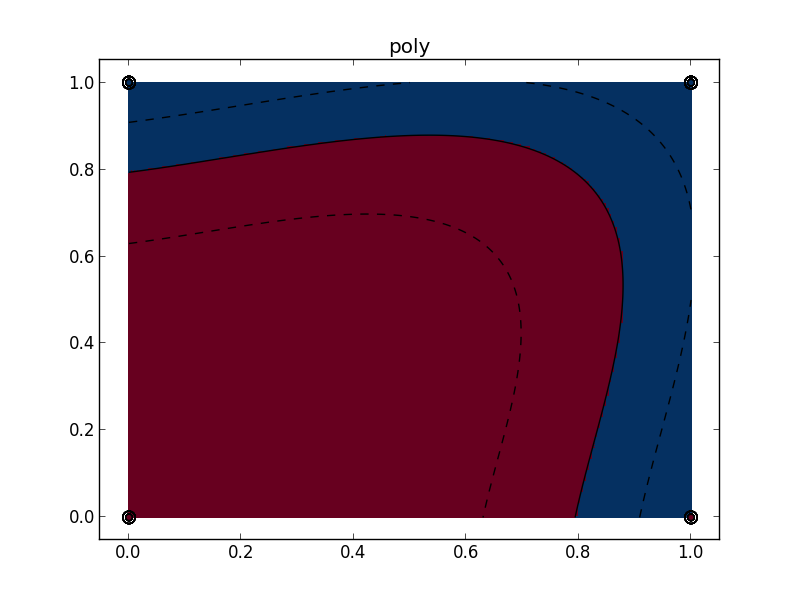
\includegraphics[width=2.4in]{eps/test_SVM_poly.png}
\caption{poly kernel}
\label {fig:pre}
\end{figure}

Any value in the blue survived while anyone in the red did not. The graph for the linear transformation creates its decision boundary right on 50\%, which contribute to the guess from earlier. The remaining decision boundaries are much more complex than the original linear decision boundary. These more complex boundaries may be able to capture more structure in the dataset, if that structure exists, and so might create a more powerful predictive model.\\


\subsection{Random Forest}
Random forests are an ensemble learning method for classification (and regression) that operate by constructing a multitude of decision trees at training time and outputting the class that is the mode of the classes output by individual trees. This technique is a form of non-parametric modeling that does away with all those equations we created above, and uses raw computing power and a clever statistical observation to tease the structure out of the data.

%----------------------------------------------------------------------------------------
%	SECTION 3
%----------------------------------------------------------------------------------------


\section{Possible results}

SVM and Random Forest are supposed to perform better than Logit model, maybe could get an accuracy more than 0.8

\end{document}